% Provenance (never printed): see sources/outline_sources.md (Year 2: Hadean, Archean and
% Proterozoic; early crust and greenstone belts; the oxygenation of the atmosphere; snowball
% Earth). Eons and eras from the ICS chart; greenstone belts, TTG and cratons after Cawood and
% others (2018) and Smithies and others (2019); komatiite liquidus after Sossi and O'Neill (2016),
% Pierru and others (2022) and Asimow (2022); the Archean air and the GOE after Catling and Zahnle
% (2020) and Luo and others (2016); the boring billion after Lyons and others (2021); snowball
% Earth after Hoffman and others (2017). The energy-balance model, the komatiite line and the CO2
% build-up from figdata/bachelor-2/precambrian.py; exercise and problem values in the Book 4
% scratch calculator calc/ch18.py.
\chapter{Bumi Prakambrium}\label{ch:b2:precambrian-earth}

Fosil bercangkang pertama muncul dalam batuan berumur sekitar 540 juta tahun. Segala sesuatu sebelumnya, sejak
lahirnya Bumi \qty{4567}{Ma} yang lalu, adalah Prakambrium: tujuh perdelapan sejarah
planet itu. Dalam waktu itu Bumi membangun inti benua-benuanya, mengisi udaranya dengan oksigen,
dan sedikitnya dua kali membeku dari kutub sampai khatulistiwa, dengan lembaran es yang mencapai laut
di daerah tropis. Bab ini membaca empat miliar tahun itu dalam batuan yang tersisa darinya,
dan menyatakan dalam angka tiga teka-tekinya: mengapa lava tertua begitu panas, bagaimana planet yang membeku
dapat mencair, dan bagaimana Bumi muda tetap hangat di bawah Matahari yang redup.
% ledger: ics:base.Hadean, ics:base.Phanerozoic, hoffman17:cryochrons

\begin{recall}
\textbf{Dari volume-volume sekolah}: umur Bumi; eon-eon pada skala waktu geologi;
hukum luminositas Matahari muda dan \omterm{def:b2:precambrian-earth:faint-sun}{masalah Matahari muda yang redup}; atmosfer purba;
stromatolit, \omterm{def:b2:precambrian-earth:bif}{formasi besi berpita}, \omterm{def:b2:precambrian-earth:goe}{Peristiwa Oksidasi Besar}, dan lapisan merah; \omterm{def:b2:precambrian-earth:craton}{kraton};
kalor radiogenik pada masa lalu. \textbf{Dari volume Tahun 1}: zirkon dan umur U--Pb-nya,
suhu penutupan; produksi kalor radiogenik keempat isotop; radiasi gelombang panjang keluar
dan insolasi rata-rata global $S_0/4$; satuan kronostratigrafi.
\textbf{Dari bab-bab sebelumnya}: \omterm{def:b2:mantle-melting:tp}{suhu potensial mantel} dan adiabat
(\cref{ch:b2:mantle-melting}); likuidus dan \omterm{def:b2:magmatic-differentiation:crystallisation}{kristalisasi fraksional} olivin
(\cref{ch:b2:magmatic-differentiation}); jenis-jenis granit (\cref{ch:b2:crustal-melting});
\omterm{def:b2:wilson-cycle:supercontinent}{superbenua} (\cref{ch:b2:wilson-cycle}). Oksidasi dan reduksi termasuk buku-buku
kimia, dan eukariota pertama serta fotosintesis termasuk buku-buku biologi.
\end{recall}

\section{Tiga eon sebelum fosil}\label{sec:b2:precambrian-earth:eons}

\begin{definition}[Hadean, Arkean, Proterozoikum]\label{def:b2:precambrian-earth:eons}
Waktu sebelum Fanerozoikum dibagi menjadi tiga eon. \emph{Hadean}\index{Hadean}
berlangsung dari pembentukan Bumi, \qty{4567}{Ma} yang lalu, sampai $4031 \pm \qty{3}{Ma}$;
\emph{Arkean}\index{Arkean} dari $4031$ sampai \qty{2500}{Ma}; dan
\emph{Proterozoikum}\index{Proterozoikum} dari 2500 sampai \qty{538.8}{Ma}, dasar Kambrium.
Bersama-sama, ketiganya secara tidak resmi disebut Prakambrium.
\end{definition}
% ledger: ics:base.Hadean, ics:base.Archean, ics:base.Proterozoic, ics:base.Phanerozoic

\omterm{def:b2:precambrian-earth:eons}{Arkean} dibagi menjadi empat era, yaitu Eoarkean (4031 sampai \qty{3600}{Ma}), Paleoarkean (3600
sampai 3200), Mesoarkean (3200 sampai 2800), dan Neoarkean (2800 sampai 2500); \omterm{def:b2:precambrian-earth:eons}{Proterozoikum} menjadi tiga,
yaitu Paleoproterozoikum (2500 sampai \qty{1600}{Ma}), Mesoproterozoikum (1600 sampai 1000), dan
Neoproterozoikum (1000 sampai 538.8). Dua periode Neoproterozoikum penting di bawah, yaitu Kriogenian, 720 sampai
\qty{635}{Ma}, dan Ediakaran, 635 sampai \qty{538.8}{Ma}.
% ledger: ics4:archean-eras, ics4:proterozoic-eras

\begin{omfigure}
\centering
% ledger: ics:base.Hadean, ics:base.Archean, ics:base.Proterozoic, ics:base.Phanerozoic, ics4:archean-eras, ics4:proterozoic-eras, wilde01:4404, bowring99:acasta, cz20:impacts, allwood06:spc, cawood18:transition, gumsley17:goe, luo16:goe, hoffman17:earlier, earle:bif, lyons21:boring, hoffman17:ages, asimow22:komatiite
\begin{tikzpicture}[x=-3.4cm, y=1cm, font=\scriptsize]
% eons
\fill[icsHadean] (4.567,0) rectangle (4.031,0.5);
\fill[icsArchean] (4.031,0) rectangle (2.5,0.5);
\fill[icsProterozoic] (2.5,0) rectangle (0.5388,0.5);
\fill[icsPhanerozoic] (0.5388,0) rectangle (0,0.5);
\node[text=white] at (4.299,0.25) {Hadean};
\node[text=white] at (3.27,0.25) {Arkean};
\node[text=white] at (1.52,0.25) {Proterozoikum};
\node at (0.27,0.25) {Fan.};
% eras
\foreach \a/\b/\c in {4.031/3.6/35, 3.6/3.2/55, 3.2/2.8/35, 2.8/2.5/55}
  \fill[icsArchean!\c] (\a,-0.45) rectangle (\b,0);
\foreach \a/\b/\c in {2.5/1.6/35, 1.6/1.0/55, 1.0/0.5388/35}
  \fill[icsProterozoic!\c] (\a,-0.45) rectangle (\b,0);
\foreach \x/\l in {3.8155/Eo, 3.4/Paleo, 3.0/Meso, 2.65/Neo, 2.05/Paleo, 1.3/Meso, 0.769/Neo}
  \node at (\x,-0.225) {\l};
% axis
\draw (4.6,-0.6) -- (0,-0.6);
\foreach \t in {0,0.5,...,4.5} {
  \draw (\t,-0.6) -- (\t,-0.7);
  \node[anchor=north] at (\t,-0.7) {\pgfmathprintnumber[fixed, precision=1]{\t}};
}
\node[anchor=north, font=\small] at (2.3,-1.05) {waktu sebelum kini (miliar tahun)};
% row A
\fill[omDef] (4.404,0.85) circle (2pt);
\node[anchor=west, text=omDef] at (4.404,0.85) {zirkon tertua};
\fill[omMeth] (3.43,0.85) circle (2pt);
\node[anchor=west, text=omMeth] at (3.43,0.85) {stromatolit pertama};
\draw[red!60!black, line width=3pt] (2.4,0.85) -- (1.8,0.85);
\node[anchor=west, text=red!60!black] at (1.8,0.85) {formasi besi berpita};
% row B
\fill[omDef] (4.03,1.5) circle (2pt);
\node[anchor=west, text=omDef] at (4.03,1.5) {batuan tertua};
\draw[black!70, line width=3pt] (3.2,1.5) -- (2.5,1.5);
\node[anchor=south, text=black!80] at (2.85,1.6) {perubahan gaya tektonik};
\draw[omProp, line width=3pt] (1.8,1.5) -- (0.8,1.5);
\node[anchor=south, text=omProp] at (1.3,1.6) {``semiliar tahun yang membosankan''};
% row C
\draw[black!60, line width=2pt, densely dashed] (4.2,2.25) -- (3.5,2.25);
\node[anchor=south, text=black!70] at (3.85,2.35) {pengeboman berat akhir? (diperdebatkan)};
\draw[omThm, line width=3pt] (2.43,2.25) -- (2.06,2.25);
\node[anchor=west, text=omThm] at (2.06,2.25) {Peristiwa Oksidasi Besar};
% row D
\fill[blue!60!black] (2.4,3.0) circle (2pt);
\node[anchor=east, text=blue!60!black] at (2.4,3.0) {Bumi bola salju pertama};
\fill[omThm] (0.8,3.0) circle (2pt);
\node[anchor=east, text=omThm] at (0.8,3.0) {kenaikan oksigen kedua};
% row E
\fill[orange!80!black] (1.9,3.7) circle (2pt);
\node[anchor=east, text=orange!80!black] at (1.9,3.7) {komatiit umum terakhir};
\draw[blue!60!black, line width=3pt] (0.717,3.7) -- (0.635,3.7);
\node[anchor=east, text=blue!60!black] at (0.717,3.7) {bola salju Kriogenian};
% row F
\fill[omMeth] (0.57,4.4) circle (2pt);
\node[anchor=east, text=omMeth] at (0.57,4.4) {fosil besar pertama (Ediakaran)};
\end{tikzpicture}
\par\smallskip{\small Prakambrium dalam satu garis. Eon-eon dan, dengan warna yang lebih muda, era-eranya
(Eo-, Paleo-, Meso-, dan Neoarkean; Paleo-, Meso-, dan Neoproterozoikum) adalah eon dan era
Bagan Kronostratigrafi Internasional; peristiwa-peristiwa ditempatkan pada umur yang dikutip dalam teks.
``\omterm{def:b2:precambrian-earth:greenstone}{Komatiit} umum terakhir'' adalah \omterm{def:b2:precambrian-earth:greenstone}{komatiit} yang tidak terkuras aluminiumnya; jenis yang lebih muda dan lebih langka ada.}
\end{omfigure}

\subsection*{Hadean: mineral tanpa batuan}

Tidak ada batuan yang tersisa dari \omterm{def:b2:precambrian-earth:eons}{Hadean}, hanya mineral. Yang tertua adalah sebutir zirkon dari Jack
Hills di Australia Barat, berumur $4404 \pm \qty{8}{Ma}$, yang tercuci keluar dari batuan yang lebih tua dan diendapkan
dalam konglomerat sekitar tiga miliar tahun yang lalu. Komposisinya, dan komposisi butir-butir
tetangganya, dibaca oleh para penemunya sebagai bukti bahwa kerak bertipe benua dan
air cair sudah ada \qty{4.4}{Ga} yang lalu, sekitar 160 juta tahun setelah Bumi
terbentuk. Batuan tertua yang telah ditentukan umurnya, gneis Acasta di Kanada barat laut, berumur 4.00 sampai
\qty{4.03}{Ga}, dekat dengan dasar \omterm{def:b2:precambrian-earth:eons}{Arkean}.
% ledger: wilde01:4404, wilde01:zircon, uw14:jack-hills, bowring99:acasta

Bumi muda ditumbuk oleh benda-benda besar, seperti yang diuraikan \cref{ch:b2:planet-formation-meteorites}.
Tumbukan terakhir yang cukup besar untuk menguapkan
seluruh samudra diperkirakan terjadi sekitar \qty{4.3}{Ga} yang lalu. ``Pengeboman berat
akhir'' yang lebih kemudian, yaitu lonjakan tumbukan antara sekitar 4.2--4.0 dan \qty{3.5}{Ga} yang disimpulkan dari
umur batuan Bulan dan umur kejutan dalam \omterm{def:b2:planet-formation-meteorites:fall-find}{meteorit}, telah diajukan; banyak yang membantah bahwa peristiwa itu
merupakan peristiwa tersendiri, dan bagaimanapun juga peristiwa itu mungkin tidak akan memandulkan Bumi.
% ledger: cz20:impacts

\section{Kerak Arkean}\label{sec:b2:precambrian-earth:archean}

\subsection*{Sabuk batu hijau dan komatiit}

Kerak \omterm{def:b2:precambrian-earth:eons}{Arkean} yang tersisa terdiri atas dua jenis medan, berdampingan: tubuh-tubuh besar gneis
granitik kelabu yang kaya natrium, dan sabuk-sabuk yang lebih sempit dari batuan vulkanik dan sedimen yang teralterasi.

\begin{definition}[Sabuk batu hijau; komatiit]\label{def:b2:precambrian-earth:greenstone}
Yang disebut \emph{sabuk batu hijau}\index{sabuk batu hijau} adalah sabuk batuan vulkanik mafik dan ultramafik,
bersama sedimen, yang termetamorfosis berderajat rendah (warna hijaunya berasal dari klorit, aktinolit, dan
epidot), yang terletak di antara tubuh-tubuh granitoid di medan \omterm{def:b2:precambrian-earth:eons}{Arkean} dan sebagian medan \omterm{def:b2:precambrian-earth:eons}{Proterozoikum}. Yang disebut
\emph{komatiit}\index{komatiit} adalah lava ultramafik, jauh lebih kaya MgO daripada basal,
yang dierupsikan sebagai cairan; olivinnya biasanya tumbuh sebagai bilah-bilah panjang dan tipis, yaitu tekstur
\emph{spinifex}, selagi bagian atas aliran mendingin dengan cepat.
\end{definition}
% ledger: cawood18:dome-keel, so16:liquidus, pierru22:komatiite

\begin{omfigure}
\centering
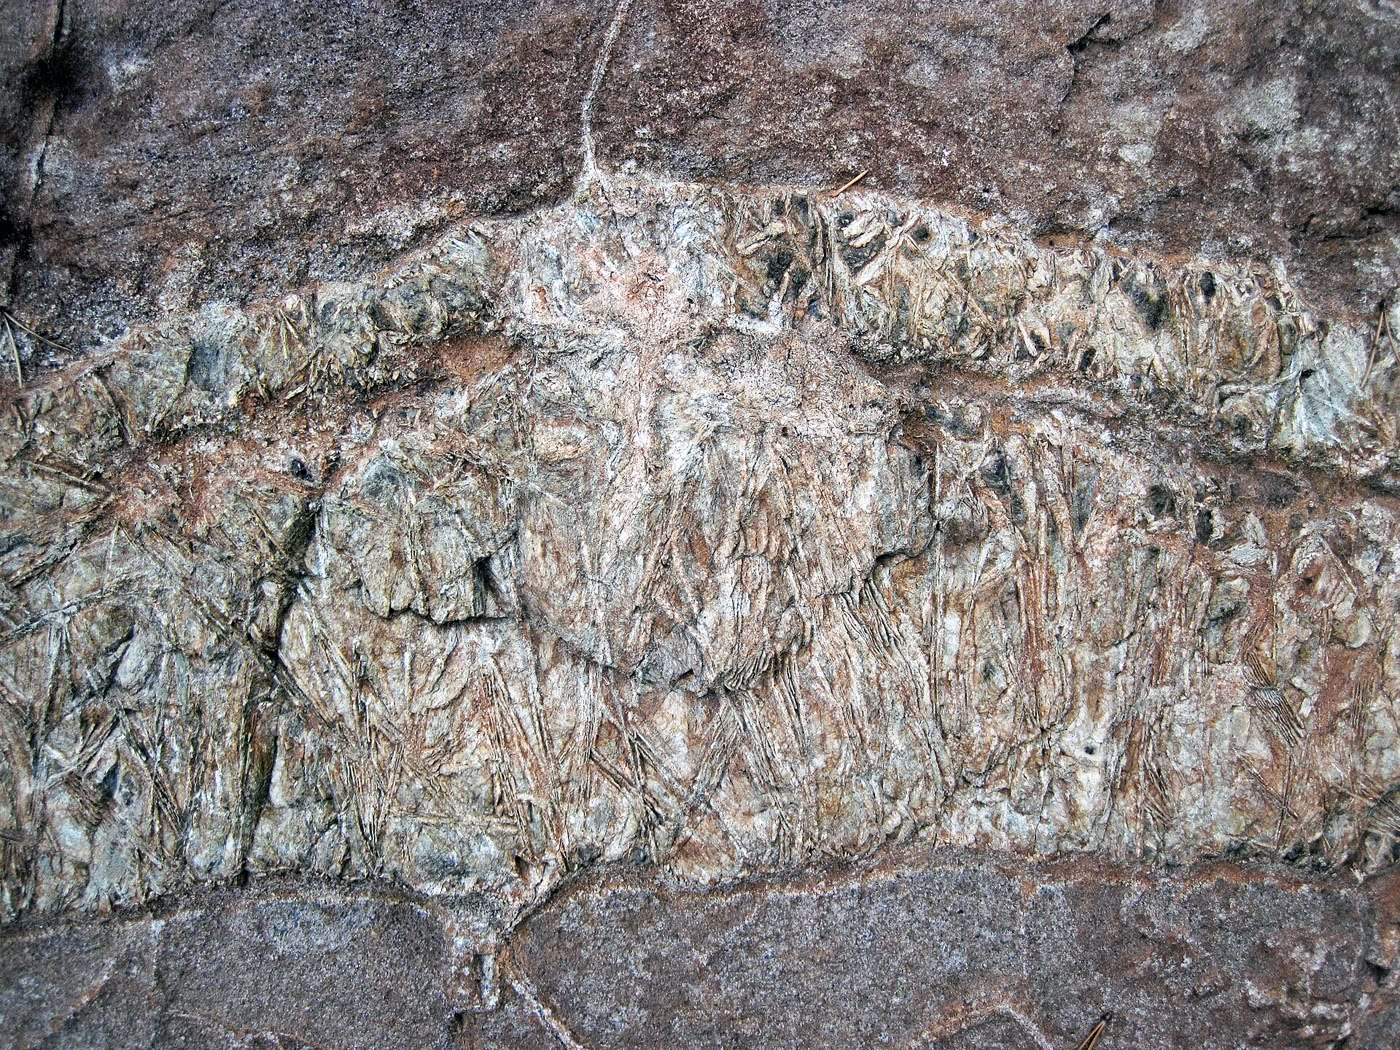
\includegraphics[width=0.66\linewidth]{images/book4/b2-18-spinifex-komatiite.jpg}
\par\smallskip{\small Tekstur spinifex dalam aliran \omterm{def:b2:precambrian-earth:greenstone}{komatiit}, Pyke Hill, Ontario, bagian dari
\omterm{def:b2:precambrian-earth:greenstone}{sabuk batu hijau} Neoarkean yang berumur sekitar 2.71 miliar tahun: bilah-bilah olivin, yang kini teralterasi,
tumbuh melintasi bagian atas aliran yang mendingin. Foto: James St.~John, CC~BY~2.0 (Wikimedia
Commons).}
\end{omfigure}

\omterm{def:b2:precambrian-earth:greenstone}{Komatiit} mengandung sampai \qty{34}{\percent} MgO, dibandingkan dengan 10 sampai \qty{13}{\percent} dalam basal
primer punggungan masa kini, dan \omterm{def:b2:precambrian-earth:greenstone}{komatiit} hampir terbatas pada Bumi tua: jenis yang terkuras aluminium
hanya ditemukan dalam batuan yang lebih tua daripada \qty{2.8}{Ga}, jenis yang tidak terkuras aluminium sampai sekitar
\qty{1.9}{Ga}, dan hanya jenis langka yang diperkaya aluminium yang semuda \qty{90}{Ma}. Lelehan
yang begitu kaya magnesium sangat panas, dan, seperti pada basal di
\cref{ch:b2:magmatic-differentiation}, mineral pertama yang mengkristal darinya adalah olivin,
yang bagiannya dalam cairan menentukan suhu.
% ledger: pierru22:komatiite, asimow22:komatiite

\begin{proposition}[Termometer komatiit]\label{prop:b2:precambrian-earth:liquidus}
Untuk lelehan yang setimbang dengan olivin pada tekanan atmosfer, suhu likuidus naik
hampir linear terhadap kandungan MgO lelehan itu. Melalui dua eksperimen $(m_1, T_1)$ dan
$(m_2, T_2)$,
\[
  T_{\text{liq}}(m) = T_1 + s\,(m - m_1), \qquad s = \frac{T_1 - T_2}{m_1 - m_2} .
\]
Eksperimen pelelehan pada dua \omterm{def:b2:precambrian-earth:greenstone}{komatiit}, $\qty{32.2}{\percent}$ MgO pada \qty{1616}{\celsius} dan
$\qty{23}{\percent}$ pada \qty{1450}{\celsius}, memberikan $s = \qty{18.0}{\celsius}$ per persen
MgO.
\end{proposition}
% ledger: so16:liquidus, helz98:glass-thermometer

\begin{proof}
Olivin adalah larutan padat forsterit dan fayalit, jauh lebih kaya magnesium daripada lelehan
tempat olivin itu tumbuh. Selagi lelehan mendingin, olivin mengambil magnesium darinya, dan suhu
saat lelehan tepat jenuh olivin turun bersama kandungan MgO-nya. Eksperimen menunjukkan bahwa
dalam rentang satu keluarga lelehan, penurunan itu hampir linear, sehingga garis yang melalui
dua eksperimen menginterpolasi di antara keduanya; $s = (1616 - 1450)/(32.2 - 23) = 166/9.2 = 18.04$.
\end{proof}

Koefisien itu tidak khas bagi \omterm{def:b2:precambrian-earth:greenstone}{komatiit}. Kaca yang dicelup cepat dari lava Kilauea,
yang dikalibrasi dengan cara yang sama, berubah sebesar \qty{3}{\celsius} untuk \qty{0.15}{\percent} MgO, yaitu
\qty{20}{\celsius} per persen. Memperpanjang garis \omterm{def:b2:precambrian-earth:greenstone}{komatiit} ke bawah sampai basal punggungan primer
dengan \qty{12}{\percent} MgO dengan demikian memberikan likuidusnya dalam selisih beberapa puluh derajat: $1616 -
18.0\times20.2 \approx \qty{1252}{\celsius}$. Jadi cairan \omterm{def:b2:precambrian-earth:greenstone}{komatiit} terpanas
sekitar \qty{360}{\celsius} lebih panas daripada lelehan yang memasok punggungan masa kini, dan gambar di bawah
menunjukkan garis itu.
% ledger: helz98:glass-thermometer, so16:liquidus, pierru22:komatiite
% values: slope 18.043, T_morb12 1251.5, dT_kom_morb 364.5 (precambrian.py)

\begin{omfigure}
\centering
\begin{tikzpicture}
\begin{axis}[omrecord, width=0.72\linewidth, height=6cm, xmin=8, xmax=35, ymin=1150, ymax=1700,
  xlabel={MgO dalam lelehan (\unit{\percent} massa)}, ylabel={likuidus pada 1 atm (\unit{\celsius})},
  xtick pos=bottom, ytick pos=left, clip=false,
  y tick label style={/pgf/number format/1000 sep={}}]
% computed in figdata/bachelor-2/precambrian.py part kom; ledger: so16:liquidus, pierru22:komatiite
\fill[omProp!15] (axis cs:10,1150) rectangle (axis cs:13,1700);
\addplot[black, line width=1.1pt] table[x=MgO, y=T] {figdata/out/bachelor-2-precambrian-kom.dat};
\addplot[only marks, mark=*, mark size=2.4pt, omThm] coordinates {(32.2,1616) (23,1450)};
\node[anchor=north west, font=\scriptsize, text=omThm] at (axis cs:32.2,1612) {Barberton};
\node[anchor=north west, font=\scriptsize, text=omThm] at (axis cs:23,1446) {Munro};
\node[anchor=south, font=\scriptsize, text=omProp, align=center] at (axis cs:11.5,1560)
  {basal punggungan\\primer};
\draw[densely dashed] (axis cs:12,1150) -- (axis cs:12,1251.5) -- (axis cs:8,1251.5);
\draw[densely dashed] (axis cs:32.2,1150) -- (axis cs:32.2,1616);
\draw[<->, omDef, thick] (axis cs:27,1251.5) -- (axis cs:27,1616);
\draw[densely dotted] (axis cs:12,1251.5) -- (axis cs:27,1251.5);
\draw[densely dotted] (axis cs:27,1616) -- (axis cs:32.2,1616);
\node[anchor=east, font=\scriptsize, text=omDef] at (axis cs:26.7,1330) {sekitar \qty{360}{\celsius}};
\end{axis}
\end{tikzpicture}
\par\smallskip{\small Termometer \omterm{def:b2:precambrian-earth:greenstone}{komatiit}: garis yang melalui suhu likuidus
yang diukur pada dua \omterm{def:b2:precambrian-earth:greenstone}{komatiit} (titik), diperpanjang sampai 10 sampai \qty{13}{\percent} MgO
basal primer punggungan masa kini (pita). Perpanjangan itu bertumpu pada kemiripan kemiringan lelehan basaltik.}
\end{omfigure}

Lava yang lebih panas tidak berarti mantel yang lebih panas dengan besaran yang sama. \omterm{def:b2:precambrian-earth:greenstone}{Komatiit} mungkin naik dalam
plume, seperti basal terpanas masa kini di Hawaii, tempat suhu potensial mencapai
sekitar \qty{200}{\celsius} di atas $1350 \pm \qty{50}{\celsius}$ mantel sekitarnya. Dan
\omterm{def:b2:precambrian-earth:greenstone}{komatiit} terbentuk oleh derajat pelelehan yang besar, pada kedalaman yang lebih besar. \omterm{def:b2:precambrian-earth:greenstone}{Komatiit} umumnya dianggap
terbentuk dalam mantel yang 200 sampai \qty{300}{K} lebih hangat daripada mantel kini; pandangan alternatif menyatakan bahwa
\omterm{def:b2:precambrian-earth:greenstone}{komatiit} adalah \omterm{def:b2:magma-emplacement:magma}{magma} basah, yang terbentuk pada suhu yang tidak jauh lebih tinggi daripada mantel
di sekitarnya. Bagaimanapun juga, mantel \omterm{def:b2:precambrian-earth:eons}{Arkean} lebih panas, dan volume-volume
sekolah memberikan satu alasan: 3 miliar tahun yang lalu keempat isotop radioaktif melepaskan lebih dari
dua kali kalor masa kini (\cref{exo:b2:precambrian-earth:2}).
% ledger: asimow22:komatiite, pierru22:komatiite, so16:liquidus

\subsection*{TTG dan pola kubah dan lunas}

Gneis kelabu di antara sabuk-sabuk batu hijau bukanlah granit dari jenis yang
diuraikan \cref{ch:b2:crustal-melting}.

\begin{definition}[Rangkaian tonalit--trondhjemit--granodiorit]\label{def:b2:precambrian-earth:ttg}
Yang disebut \emph{rangkaian tonalit--trondhjemit--granodiorit}\index{rangkaian tonalit--trondhjemit--granodiorit}
(TTG) adalah keluarga granitoid yang kaya natrium dan miskin kalium --- tonalit,
trondhjemit (tonalit yang miskin mineral mafik), dan granodiorit --- yang membentuk sebagian besar
kerak benua \omterm{def:b2:precambrian-earth:eons}{Arkean}. Sebagian besar terbentuk oleh \omterm{def:b2:mantle-melting:melting}{pelelehan sebagian} kerak basaltik
yang terhidrasi.
\end{definition}
% ledger: smithies19:ttg, cawood18:ttg

Sebagian besar volume kerak benua masa kini telah terbentuk pada akhir \omterm{def:b2:precambrian-earth:eons}{Arkean}, sebagian besar
sebagai TTG. Sebagian TTG membawa tanda \omterm{def:b2:elements-in-the-earth:trace}{unsur jejak} yang lama dibaca sebagai pelelehan pada kedalaman lebih dari
\qty{50}{km}, tekanan yang tidak dicapai dalam kerak benua yang lebih muda, dan tafsiran ini
ikut berperan dalam perdebatan tentang saat dimulainya tektonik lempeng; sebuah studi tahun 2019 berpendapat bahwa tanda-tanda itu
justru berasal dari lelehan mantel, dan bahwa TTG yang umum terbentuk pada
kedalaman yang tidak lebih besar daripada \qty{40}{km} kerak benua biasa masa kini. Menjelang akhir
\omterm{def:b2:precambrian-earth:eons}{Arkean}, antara sekitar 3.0 dan \qty{2.5}{Ga}, granitoid sebagian besar \omterm{def:b2:precambrian-earth:craton}{kraton} berubah dari TTG
menjadi granit kaya kalium, tanda kerak yang lebih tebal yang dilelehkan kembali.
% ledger: smithies19:ttg, cawood18:ttg

Di Pilbara timur di Australia, di Zimbabwe, dan di India selatan, kedua medan itu menggambar
pola yang mencolok pada peta. Kubah-kubah granitoid yang membundar dibingkai oleh lunas-lunas sinklin batu hijau yang lapisannya miring dan menghadap menjauhi kubah. Kubah-kubah itu
diduga naik sebagai \omterm{def:b2:magma-emplacement:ascent}{diapir}, kerak granitik yang ringan yang naik menembus tumpukan tebal dan padat
lava yang tenggelam di antaranya. Di Pilbara pembentukan kubah ini berlangsung selama ratusan juta
tahun dan berhenti sekitar \qty{3.1}{Ga} yang lalu, setelah itu struktur-strukturnya menjadi linear, seperti struktur
\omterm{def:b2:alpine-orogen:orogen}{orogen} yang lebih muda.
% ledger: cawood18:dome-keel

\begin{omfigure}
\centering
\begin{tikzpicture}[x=0.95cm, y=0.95cm, font=\scriptsize]
% schematic, after the description in cawood18:dome-keel
\fill[lith basalt] (0,0) rectangle (12,7);
\draw (0,0) rectangle (12,7);
\foreach \cx/\cy/\rx/\ry in {2.4/4.7/1.7/1.4, 7.2/5.0/2.0/1.4, 4.6/1.6/1.9/1.1, 10.0/2.0/1.4/1.3}
  \filldraw[lith granite, draw=black, thick] (\cx,\cy) ellipse ({\rx} and {\ry});
% strike and dip in the greenstone, each dipping away from the nearest dome
% (positions and strikes from the outward normals of the ellipses, computed by hand)
\foreach \px/\py/\st in {3.9/5.99/309, 0.9/5.99/231, 0.9/3.41/129, 2.4/2.88/90, 4.52/4.7/0,
    9.62/5.0/0, 8.91/6.29/305, 5.49/6.29/235, 8.91/3.71/55, 5.49/3.71/125,
    6.92/1.6/0, 4.6/3.12/270, 2.28/1.6/180, 6.24/0.53/60,
    10.0/3.72/270, 11.29/0.78/47, 8.18/2.0/180, 11.29/3.22/313}
  \pic at (\px,\py) {strikedip={\st}{}};
\node[fill=white, inner sep=1.5pt] at (2.4,4.7) {kubah TTG};
\node[fill=white, inner sep=1.5pt] at (7.2,5.0) {kubah TTG};
\node[fill=white, inner sep=1.5pt] at (4.6,1.6) {kubah TTG};
\node[fill=white, inner sep=1.5pt] at (10.0,2.0) {kubah TTG};
\node[fill=white, inner sep=1.5pt, align=center] at (7.45,2.75) {lunas\\batu hijau};
\node[fill=white, inner sep=1.5pt, align=center] at (1.0,0.9) {batu hijau};
\pic at (11.4,5.6) {northarrow};
% section below
\begin{scope}[yshift=-3.3cm]
\fill[lith basalt] (0,0) -- (12,0) -- (12,2.2) -- (0,2.2) -- cycle;
\filldraw[lith granite, draw=black, thick] (0.6,0) .. controls (0.6,2.0) and (4.6,2.0) .. (4.6,0) -- cycle;
\filldraw[lith granite, draw=black, thick] (6.4,0) .. controls (6.4,2.1) and (11.0,2.1) .. (11.0,0) -- cycle;
\draw[thick] (0,0) rectangle (12,2.2);
\draw[black!70] (4.6,0.9) .. controls (5.5,0.2) .. (6.4,0.9);
\draw[black!70] (4.35,1.5) .. controls (5.5,0.6) .. (6.65,1.5);
\node[fill=white, inner sep=1.5pt] at (2.6,0.6) {TTG};
\node[fill=white, inner sep=1.5pt] at (8.7,0.6) {TTG};
\node[fill=white, inner sep=1.5pt] at (5.5,1.75) {lunas};
\draw[->, thick] (2.6,1.0) -- (2.6,1.75);
\draw[->, thick] (8.7,1.05) -- (8.7,1.8);
\draw[->, thick] (5.5,1.4) -- (5.5,0.95);
\node[anchor=west] at (12.1,1.1) {penampang};
\end{scope}
\node[anchor=west] at (12.1,3.5) {peta};
\end{tikzpicture}
\par\smallskip{\small Pola kubah dan lunas pada sebagian \omterm{def:b2:precambrian-earth:craton}{kraton} \omterm{def:b2:precambrian-earth:eons}{Arkean} (skematis, tidak
berskala). Peta: kubah-kubah granitoid rangkaian TTG yang dibingkai oleh batu hijau; simbol jurus dan kemiringan
menunjukkan lapisan batu hijau yang miring menjauhi setiap kubah. Penampang: kubah-kubah
naik selagi tumpukan batu hijau yang padat tenggelam menjadi lunas-lunas sinklin di antaranya (panah).}
\end{omfigure}

\subsection*{Kraton}

\begin{definition}[Kraton]\label{def:b2:precambrian-earth:craton}
Yang disebut \emph{kraton}\index{kraton} adalah bagian benua yang tetap stabil secara tektonik
selama lebih dari satu miliar tahun: inti kerak \omterm{def:b2:precambrian-earth:eons}{Arkean} atau \omterm{def:b2:precambrian-earth:eons}{Proterozoikum}, metamorfik dan
plutonik, yang terletak di atas akar mantel litosfer yang tebal, dingin, dan apung yang mencapai kedalaman sekitar
\qty{250}{km}.
\end{definition}
% ledger: tulane:cratons, fischer:lithosphere, cawood18:ttg

\omterm{def:b2:precambrian-earth:craton}{Kraton-kraton} menjadi stabil terutama pada Mesoarkean dan Neoarkean, dan tanda-tanda
kestabilannya tertulis dalam batuan: cekungan sedimen luas yang terletak di atasnya, seperti
Supergrup Transvaal di \omterm{def:b2:precambrian-earth:craton}{kraton} Kaapvaal (sekitar 2640 sampai \qty{2055}{Ma}) dan Supergrup Mount Bruce
di Pilbara (2775 sampai \qty{2210}{Ma}); kawanan \omterm{def:b2:magma-emplacement:bodies}{retas} lurus yang memotongnya sebagai
lempeng rapuh; dan akar tebalnya, yang diperoleh pada \omterm{def:b2:precambrian-earth:eons}{Arkean} akhir. Antara 3.2 dan
\qty{2.5}{Ga} rekaman itu juga menunjukkan tepi pasif dan \omterm{def:b2:alpine-orogen:foreland}{cekungan depan-pegunungan} tertua, sabuk
\omterm{def:b2:metamorphic-facies:metamorphism}{metamorfisme} berpasangan, dan bukti paleomagnetik bahwa \omterm{def:b2:precambrian-earth:craton}{kraton-kraton} bergerak relatif satu sama lain.
Sebuah tinjauan tahun 2018 membaca perubahan-perubahan ini sebagai awal bertahap tektonik lempeng seperti yang bekerja
kini, sambil menekankan bahwa tidak ada satu pengamatan pun yang membuktikannya; taksiran yang diterbitkan tentang awal
itu berkisar dari \omterm{def:b2:precambrian-earth:eons}{Hadean} sampai Neoproterozoikum.
% ledger: cawood18:transition, cawood18:ttg, cawood18:cratons

\begin{inthefield}[Membaca sabuk batu hijau]
Di \omterm{def:b2:precambrian-earth:greenstone}{sabuk batu hijau}, pertanyaan pertama seorang ahli geologi pemeta adalah ke mana arah atas ketika
batuan terbentuk, karena lapisannya sering tegak atau terbalik. Lava bantal memberikan jawabannya
melalui bagian atasnya yang membundar dan dasar runcing yang didorongnya ke bantal di bawahnya; lapisan bersusun melalui
butirnya yang menghalus ke atas; dan aliran \omterm{def:b2:precambrian-earth:greenstone}{komatiit} melalui zonasinya, bagian atas yang terdinginkan cepat dan retak dengan
bilah-bilah spinifex yang tumbuh ke bawah ke dalamnya, di atas dasar yang kaya kristal olivin yang menumpuk. Arah
menghadap yang dipetakan dari stasiun ke stasiun menggambar sinklin-sinklin lunas. Zirkon dari tuf felsik
dan dari TTG kubah lalu memberikan umur U--Pb, sehingga ahli geologi dapat mengetahui batu hijau mana
yang lebih tua daripada kubah yang kini menerobosnya.
\end{inthefield}
% ledger: so16:liquidus (spinifex in the top zones of flows), cawood18:dome-keel

\section{Oksigen}\label{sec:b2:precambrian-earth:oxygen}

\subsection*{Udara Arkean tanpa oksigen}

Atmosfer purba volume-volume sekolah kaya nitrogen dan karbon dioksida serta
miskin oksigen. Proksi dan model kini membatasinya lebih ketat. Sebelum \qty{2.4}{Ga} oksigen
di permukaan kurang dari sepersejuta oksigen kini; karbon dioksida mungkin 10 sampai 2500
kali nilai kini dan metana 100 sampai \num{10000} kali. Butir-butir uraninit dan pirit, yang
dihancurkan oleh oksigen, dibawa oleh sungai-sungai \omterm{def:b2:precambrian-earth:eons}{Arkean} dan diendapkan tanpa teralterasi; pada \qty{2.415}{Ga}
bertahannya uraninit detritus membatasi oksigen sampai \qty{3.2e-5}{atm}. Siklus karbon, yang diingat kembali
di bawah, menjaga suhu permukaan rata-rata antara sekitar 0 dan \qty{40}{\celsius}.
% ledger: cz20:archean-air, kasting25:indicators

Oksigen sedang dibuat: sianobakteri melepaskannya melalui fotosintesis, dan jejak-jejak tipisnya muncul dalam
sebagian batuan \omterm{def:b2:precambrian-earth:eons}{Arkean}. Tetapi oksigen itu terpakai secepat terbentuknya, oleh gas vulkanik dan oleh besi
yang terlarut di laut.
% ledger: luo16:goe, lyons21:boring

\begin{definition}[Formasi besi berpita]\label{def:b2:precambrian-earth:bif}
Yang disebut \emph{formasi besi berpita}\index{formasi besi berpita} (BIF) adalah sedimen kimia berupa
lapisan-lapisan tipis yang berselang-seling antara oksida besi --- hematit, magnetit --- dan rijang. Formasi itu mengendap
dari air laut yang membawa besi(II) terlarut, ketika besi itu teroksidasi menjadi besi(III) yang tidak larut;
karena itu formasi itu memerlukan samudra dalam tanpa oksigen, pasokan besi, dan oksidator
di tempat besi diendapkan.
\end{definition}
% ledger: earle:bif, holland06:stages

\omterm{def:b2:precambrian-earth:bif}{Formasi besi berpita} paling melimpah dari 2.4 sampai \qty{1.8}{Ga}; setelah itu samudra dalam
tidak lagi membawa cukup besi terlarut, dan formasi itu pada dasarnya lenyap, lalu kembali sebentar dalam
endapan glasial Kriogenian (di bawah). Formasi itu adalah bijih besi yang umum
(\cref{ch:b2:ore-deposits}).
% ledger: earle:bif, hoffman17:models

\subsection*{Peristiwa Oksidasi Besar}

\begin{definition}[Peristiwa Oksidasi Besar]\label{def:b2:precambrian-earth:goe}
Yang disebut \emph{Peristiwa Oksidasi Besar}\index{Peristiwa Oksidasi Besar} (GOE) adalah selang, dari sekitar
2.4--2.3 sampai sekitar \qty{2.1}{Ga}, ketika oksigen untuk pertama kalinya terakumulasi secara menetap di
atmosfer dan samudra dangkal, naik dari kurang dari sepersejuta tingkatnya kini sampai
mungkin sepersepuluhnya.
\end{definition}
% ledger: cz20:goe, cz20:archean-air, gumsley17:goe, holland06:stages

Penanda yang paling jelas adalah tanda isotop sulfur. Dalam sedimen yang lebih tua daripada GOE,
isotop-isotop sulfur terpilah dengan cara yang hanya dihasilkan oleh fotokimia dalam udara tanpa oksigen;
tanda itu lenyap ketika oksigen datang. Fisikanya dan rekamannya yang lengkap termasuk
volume Tahun 3; di sini tanda itu berfungsi sebagai jam. Dalam tiga inti bor yang menembus Supergrup
Transvaal di Afrika Selatan, tanda itu lenyap pada \qty{2.33}{Ga}, dalam 1 sampai \qty{10}{Ma}:
kenaikan itu sendiri berlangsung cepat. Rekaman lain menempatkan awal peristiwa itu pada 2.46 sampai \qty{2.43}{Ga},
pada waktu glasiasi global pertama, dan menunjukkan bahwa oksigen tidak naik secara tetap
sesudahnya.
% ledger: luo16:goe, farquhar00:sulfur, pk02:anoxic, gumsley17:goe

Setelah GOE, lapisan merah muncul, pirit dan uraninit detritus lenyap dari pasir sungai,
dan tanah menyimpan besinya sebagai oksida. Tetapi samudra dalam tetap anoksik selama lebih dari satu miliar
tahun.
% ledger: kasting25:indicators, lyons21:boring

\subsection*{``Semiliar tahun yang membosankan'' dan kenaikan kedua}

Selang dari sekitar 1.8 sampai \qty{0.8}{Ga} menunjukkan begitu sedikit perubahan dalam isotop karbon
karbonat laut sehingga selang itu luas disebut ``semiliar tahun yang membosankan''. Oksigennya diperdebatkan: taksiran
awal memberikan 1 sampai \qty{40}{\percent} tingkat kini, isotop kromium mengisyaratkan kurang dari
\qty{1}{\percent}, mungkin \qty{0.1}{\percent}. Samudra dalam anoksik. Selama selang ini
eukariota, seperti diceritakan buku-buku biologi, muncul, beranekaragam, dan bertambah jumlahnya. Sejak sekitar \qty{800}{Ma} banyak rekaman menunjukkan
kenaikan oksigen kedua yang mendadak, pada waktu perkembangan besar kehidupan kompleks; apakah
oksigen memicunya atau mengikutinya masih diperdebatkan. Fosil besar Ediakaran
muncul sejak sekitar \qty{570}{Ma}. Sementara itu \omterm{def:b2:wilson-cycle:supercontinent}{superbenua-superbenua} \cref{ch:b2:wilson-cycle}
menyatu dan pecah: tepi pasif, tanda pemisahan benua, melimpah sekitar 2100 sampai
\qty{1850}{Ma}, ketika Nuna menyatu, dan lagi dari 650 sampai \qty{500}{Ma}.
% ledger: lyons21:boring, lyons21:eukaryotes, cawood18:ttg, nance22:supercontinents

\section{Es sampai khatulistiwa}\label{sec:b2:precambrian-earth:snowball}

\subsection*{Umpan balik es--albedo}

Salju dan es memantulkan sebagian besar sinar matahari yang diterimanya, laut terbuka sangat sedikit: sekitar
\qty{6}{\percent} untuk samudra, 50 sampai \qty{70}{\percent} untuk es laut tanpa salju, sampai
\qty{90}{\percent} untuk es yang tertutup salju. Bumi yang mendingin menumbuhkan lebih banyak es, memantulkan lebih banyak
sinar matahari, dan mendingin lebih jauh.
% ledger: nsidc:albedo-ice, albedo:surfaces

\begin{definition}[Umpan balik es--albedo]\label{def:b2:precambrian-earth:ice-albedo}
Yang disebut \emph{umpan balik es--albedo}\index{umpan balik es--albedo} adalah penguatan perubahan
suhu oleh perubahan tutupan salju dan es yang ditimbulkannya: pendinginan memperluas es, yang
menaikkan albedo planet, mengurangi sinar matahari yang diserap, dan mendinginkan planet lebih jauh;
pemanasan bekerja ke arah sebaliknya. Umpan balik ini adalah umpan balik positif.
\end{definition}
% ledger: hoffman17:hysteresis, nsidc:albedo-ice

Akibat-akibatnya terlihat dalam model iklim paling sederhana, yaitu planet dengan satu suhu $T$ dan
kapasitas kalor $C$ per meter persegi. Planet itu menyerap $\tfrac14 S(1 - a)$, dengan $S$ sinar matahari
pada jaraknya dan $a$ albedonya, dan kehilangan radiasi gelombang panjang keluar dari volume
Tahun 1, yang ditulis $\varepsilon\sigma T^4$: $\varepsilon$, yaitu \emph{emisivitas efektif},
mengukur seberapa banyak pancaran permukaan yang lolos dari efek rumah kaca, dan kini nilainya
$240.2/(\sigma\times288^4) = 0.616$. Untuk memasukkan umpan balik itu, albedo dijadikan fungsi
suhu. Bab ini memilih $a = 0.294$, nilai kini, bila $T \ge \qty{283}{K}$; $a
= 0.6$, nilai yang diberikan model-model iklim untuk permukaan yang membeku secara global, bila $T \le \qty{263}{K}$; dan
garis lurus di antaranya. Kedua ambang itu adalah pilihan pemodelan, bukan besaran
yang terukur.
% ledger: earth:TSI, earth:albedo, earth:Tsurf, const:sigma, hoffman17:models
% values: eps 0.6158 (precambrian.py)

\begin{proposition}[Kesetimbangan model neraca energi]\label{prop:b2:precambrian-earth:ebm}
Dalam model
\[
  C\,\frac{\mathrm dT}{\mathrm dt} = \tfrac14 S\bigl(1 - a(T)\bigr) - \varepsilon\sigma T^4
  = R(T) - E(T),
\]
suhu-suhu tunak adalah penyelesaian $R(T) = E(T)$. Suhu tunak $T^*$
stabil jika $E'(T^*) > R'(T^*)$ dan tidak stabil jika $E'(T^*) < R'(T^*)$.
\end{proposition}

\begin{proof}
Pada penyelesaian $R = E$ ruas kanan lenyap, sehingga $T$ tetap. Di dekatnya, ambil $T = T^*
+ \delta$: sampai orde pertama $C\,\dot\delta = (R'(T^*) - E'(T^*))\,\delta$, yang penyelesaiannya
$\delta(t) = \delta(0)\,e^{(R' - E')t/C}$ meluruh bila $E' > R'$ dan tumbuh bila $E' < R'$.
\end{proof}

$E$ selalu naik bersama $T$. $R$ datar di tempat albedo tetap, sehingga kesetimbangan beku dan kesetimbangan
hangat stabil; di lereng di antara keduanya $R$ naik, karena pemanasan mencairkan es, dan jika naiknya
lebih cepat daripada $E$, kesetimbangan di situ tidak stabil. Gambar di bawah menunjukkan bahwa dengan sinar matahari
masa kini model itu memiliki tiga kesetimbangan.

\begin{example}[Tiga iklim di bawah Matahari masa kini]\label{ex:b2:precambrian-earth:three}
Dengan $S_0 = \qty{1361}{W.m^{-2}}$, kesetimbangan hangat adalah \qty{288}{K} menurut konstruksinya. Sebuah
bola salju menyerap $\tfrac14 S_0\times0.4 = \qty{136.1}{W.m^{-2}}$, sehingga $T^4 =
136.1/(0.616\,\sigma)$ dan $T = \qty{249.8}{K}$, di bawah \qty{263}{K}: keadaan beku juga
ada. Di antara keduanya, di lereng, $R = E$ lagi pada \qty{275.5}{K}, keadaan yang tidak stabil:
planet yang sedikit lebih hangat memanas sampai \qty{288}{K}, planet yang sedikit lebih dingin membeku.
\end{example}
% values: T_snow_today 249.9, T_mid_today 275.5 (precambrian.py)

\begin{omfigure}
\centering
\begin{tikzpicture}
\begin{axis}[omrecord, width=0.76\linewidth, height=6.2cm, xmin=215, xmax=305, ymin=80, ymax=280,
  xlabel={suhu permukaan rata-rata global $T$ (\unit{K})}, ylabel={fluks (\unit{W.m^{-2}})},
  xtick pos=bottom, ytick pos=left, clip=false,
  legend style={at={(0.5,1.04)}, anchor=south, draw=none, font=\scriptsize, legend columns=3}]
% computed in figdata/bachelor-2/precambrian.py part ebm; ledger: earth:TSI, earth:albedo, earth:Tsurf, const:sigma, hoffman17:models, gough81:luminosity
\fill[blue!8] (axis cs:263,80) rectangle (axis cs:283,280);
\addplot[black, line width=1.1pt, restrict x to domain=219:299] table[x=T_K, y=emit] {figdata/out/bachelor-2-precambrian-ebm.dat};
\addlegendentry{dipancarkan $E(T)$}
\addplot[omThm, line width=1.1pt] table[x=T_K, y=absS0] {figdata/out/bachelor-2-precambrian-ebm.dat};
\addlegendentry{diserap, Matahari kini}
\addplot[omDef, line width=1.1pt, densely dashed] table[x=T_K, y=absP4] {figdata/out/bachelor-2-precambrian-ebm.dat};
\addlegendentry{diserap, 4 Ga yang lalu}
\addplot[only marks, mark=*, mark size=2.4pt, black] coordinates {(249.9,136.1) (288,240.2)};
\addplot[only marks, mark=o, mark size=2.4pt, black, thick] coordinates {(275.5,204.4)};
\addplot[only marks, mark=*, mark size=2.4pt, omDef] coordinates {(231.8,100.85)};
\node[anchor=north west, font=\scriptsize] at (axis cs:250.5,134) {bola salju};
\node[anchor=south east, font=\scriptsize] at (axis cs:287.5,242) {kini};
\node[anchor=south east, font=\scriptsize] at (axis cs:275,206) {tidak stabil};
\node[anchor=north west, font=\scriptsize, text=omDef] at (axis cs:237,97.5) {satu-satunya keadaan 4 Ga yang lalu};
\node[anchor=north, font=\scriptsize, text=blue!60!black, align=center] at (axis cs:273,276)
  {es\\mundur};
\end{axis}
\end{tikzpicture}
\par\smallskip{\small Model neraca energi dalam teks: radiasi yang dipancarkan (hitam) dan
sinar matahari yang diserap di bawah Matahari kini (merah) dan di bawah Matahari 4 miliar tahun yang lalu,
yang terangnya \qty{74}{\percent} (biru, putus-putus), dengan emisivitas efektif kini. Di pita yang
diarsir, albedo turun dari 0.6 sampai 0.294 selagi es mundur. Titik penuh: kesetimbangan stabil;
titik kosong: tidak stabil.}
\end{omfigure}
% values: T_snow_4 231.8, lum_4 0.7406 (precambrian.py)

\begin{proposition}[Titik kritis]\label{prop:b2:precambrian-earth:tipping}
Dalam model ini iklim hangat hanya ada jika $S \ge S_{\text{f}}$ dan bola salju hanya jika
$S \le S_{\text{m}}$, dengan
\[
  S_{\text{f}} = \frac{4\varepsilon\sigma T_2^4}{1 - a_{\text{w}}}, \qquad
  S_{\text{m}} = \frac{4\varepsilon\sigma T_1^4}{1 - a_{\text{i}}},
\]
dengan $T_1 = \qty{263}{K}$ dan $T_2 = \qty{283}{K}$ ujung-ujung lereng dan $a_{\text{i}}$,
$a_{\text{w}}$ albedo planet yang membeku dan planet yang hangat. Di antara $S_{\text{f}}$ dan
$S_{\text{m}}$ keduanya ada.
\end{proposition}

\begin{proof}
Pada cabang hangat $a = a_{\text{w}}$ dan kesetimbangannya adalah $T_{\text{w}} = (S(1 -
a_{\text{w}})/(4\varepsilon\sigma))^{1/4}$, yang naik bersama $S$; kesetimbangan itu merupakan keadaan hangat yang sah hanya
jika $T_{\text{w}} \ge T_2$, yaitu $S \ge S_{\text{f}}$. Demikian pula kesetimbangan bola salju
$(S(1 - a_{\text{i}})/(4\varepsilon\sigma))^{1/4}$ sah hanya jika tidak melampaui $T_1$, yaitu
$S \le S_{\text{m}}$.
\end{proof}

Dengan emisivitas kini, $S_{\text{f}} = \qty{1269}{W.m^{-2}}$, \qty{93.2}{\percent} sinar matahari
kini, dan $S_{\text{m}} = \qty{1670}{W.m^{-2}}$, \qty{122.7}{\percent}. Gambar di bawah
menggambarkan kesetimbangan-kesetimbangan terhadap sinar matahari. Lipatannya membentuk simpal: Bumi hangat yang sinar mataharinya
atau efek rumah kacanya melemah melewati lipatan kiri membeku sekaligus, dan Bumi yang membeku tetap membeku
sampai didorong melewati lipatan kanan, jauh melampaui keadaan saat ia membeku. Inilah
histeresis yang digambarkan Hoffman dan kawan-kawan untuk Bumi yang sebenarnya dengan model-model yang lebih lengkap,
dengan garis es yang maju ``tanpa terkendali sampai ke khatulistiwa'' begitu garis itu mencapai ambang
ketidakstabilan.
% ledger: hoffman17:hysteresis
% values: S_freeze 1268.9, S_melt 1670.5, s_freeze 0.9323, s_melt 1.2274 (precambrian.py)

\begin{omfigure}
\centering
\begin{tikzpicture}
\begin{axis}[omrecord, width=0.76\linewidth, height=6.2cm, xmin=0.7, xmax=1.4, ymin=220, ymax=320,
  xlabel={sinar matahari $S/S_0$}, ylabel={suhu kesetimbangan (\unit{K})},
  xtick pos=bottom, ytick pos=left, clip=false, unbounded coords=jump,
  x tick label style={/pgf/number format/.cd, fixed, fixed zerofill, precision=1}]
% computed in figdata/bachelor-2/precambrian.py part branch; ledger: earth:TSI, earth:albedo, earth:Tsurf, const:sigma, hoffman17:models, gough81:luminosity
\addplot[omDef, line width=1.2pt] table[x=s, y=Tsnow] {figdata/out/bachelor-2-precambrian-branch.dat};
\addplot[black, line width=1.0pt, densely dashed] table[x=s, y=Tmid] {figdata/out/bachelor-2-precambrian-branch.dat};
\addplot[omThm, line width=1.2pt] table[x=s, y=Twarm] {figdata/out/bachelor-2-precambrian-branch.dat};
\draw[black!50, densely dotted] (axis cs:1,220) -- (axis cs:1,320);
\draw[black!50, densely dotted] (axis cs:0.7406,220) -- (axis cs:0.7406,320);
\node[anchor=south west, font=\scriptsize, rotate=90] at (axis cs:1.0,222) {kini};
\node[anchor=south west, font=\scriptsize, rotate=90] at (axis cs:0.7406,237) {4 Ga yang lalu};
\draw[->, thick, blue!60!black] (axis cs:0.9323,281) -- (axis cs:0.9323,248);
\draw[->, thick, omThm] (axis cs:1.2274,265) -- (axis cs:1.2274,300);
\node[anchor=north west, font=\scriptsize, text=omThm] at (axis cs:1.02,314) {cabang hangat};
\node[anchor=north, font=\scriptsize, text=omDef] at (axis cs:0.85,236) {cabang bola salju};
\node[anchor=south, font=\scriptsize] at (axis cs:1.12,268) {tidak stabil};
\node[anchor=east, font=\scriptsize, text=blue!60!black, align=right] at (axis cs:0.925,266) {membeku\\sekaligus};
\node[anchor=west, font=\scriptsize, text=omThm, align=left] at (axis cs:1.235,282) {mencair\\sekaligus};
\end{axis}
\end{tikzpicture}
\par\smallskip{\small Kesetimbangan model terhadap sinar matahari, pada emisivitas efektif
kini: cabang hangat (merah), cabang bola salju (biru), dan cabang tidak stabil
di antara keduanya (putus-putus). Panah-panah menandai kedua titik kritis
\cref{prop:b2:precambrian-earth:tipping}.}
\end{omfigure}

\subsection*{Matahari muda yang redup}

\begin{definition}[Masalah Matahari muda yang redup]\label{def:b2:precambrian-earth:faint-sun}
Yang disebut \emph{masalah Matahari muda yang redup}\index{masalah Matahari muda yang redup} adalah pertentangan antara
model-model Matahari, yang membuatnya 25 sampai \qty{30}{\percent} lebih redup \qty{4}{Ga} yang lalu, dan
batuan, yang menunjukkan air cair dan siklus air yang aktif sepanjang \omterm{def:b2:precambrian-earth:eons}{Arkean}: dengan atmosfer
dan albedo masa kini, Bumi awal seharusnya membeku.
\end{definition}
% ledger: cz20:archean-air, feulner12:fys, gough81:luminosity

Model neraca energi mempertajam masalah itu lebih daripada yang dapat dilakukan volume-volume sekolah. Dengan hukum
Gough, sinar matahari \qty{4}{Ga} yang lalu adalah \qty{74.1}{\percent} sinar matahari kini, di bawah
\qty{93.2}{\percent} tempat iklim hangat lenyap: dengan emisivitas kini satu-satunya
kesetimbangan adalah bola salju pada \qty{232}{K}. Hukum itu baru mencapai $0.932$ pada
\qty{0.83}{Ga} yang lalu. Jadi, selama lebih dari tiga perempat sejarahnya, Bumi dengan
udara masa kini tidak mungkin hangat, dan begitu membeku Bumi akan memerlukan lebih banyak lagi untuk mencair.
% ledger: gough81:luminosity, connelly12:cai
% values: T_snow_4 231.8, ago_freeze 0.829 (precambrian.py)

\begin{example}[Efek rumah kaca Bumi muda]\label{ex:b2:precambrian-earth:young-greenhouse}
Untuk mempertahankan \qty{288}{K} di bawah Matahari \qty{4}{Ga} yang lalu dengan albedo masa kini, sinar matahari
yang diserap adalah $0.741\times340.25\times0.706 = \qty{178.0}{W.m^{-2}}$, sehingga emisivitas efektif
harus turun menjadi $178.0/(\sigma\times288^4) = 0.456$, dibandingkan dengan 0.616 kini: bagian
pancaran permukaan yang terperangkap oleh efek rumah kaca harus naik dari 0.384 menjadi 0.544.
\end{example}
% values: eps_warm_4 0.456 (precambrian.py)

Batuan menyatakan bahwa efek rumah kaca memang lebih kuat. Karbon dioksida saja sudah cukup dengan
0.024 sampai \qty{1}{bar} \qty{4}{Ga} yang lalu dan 0.004 sampai \qty{0.03}{bar} pada \qty{2.5}{Ga}, dan
metana, yang melimpah dalam udara anoksik, ikut membantu. Sebuah termostat menjaganya demikian: pelapukan silikat,
yang memakai karbon dioksida, melambat ketika iklim mendingin dan mempercepat ketika iklim memanas, sehingga
karbon dioksida di udara menyesuaikan diri sampai iklim menjadi sedang. Termostat yang sama menjelaskan
bagaimana sebuah bola salju berakhir.
% ledger: cz20:archean-air, feulner12:fys

\subsection*{Bumi bola salju}

Endapan glasial Neoproterozoikum --- diamiktit, permukaan batuan dasar bergores, batu yang jatuh dari
es terapung ke dalam sedimen halus --- menunjukkan lembaran es yang bertumpu di dasar dan mencapai laut di semua lintang,
dan paleomagnetisme, yang dibahas volume Tahun 3, menempatkan beberapa di antaranya di dekat khatulistiwa. Glasiasi Sturtian,
misalnya, dimulai pada paleolintang $21 \pm \ang{3}$\,LU, di wilayah Yukon kini.
% ledger: hoffman17:cryochrons, hoffman17:ages, hoffman17:deposits

\begin{definition}[Bumi bola salju; karbonat penudung]\label{def:b2:precambrian-earth:snowball}
Yang disebut \emph{Bumi bola salju}\index{Bumi bola salju} adalah keadaan Bumi ketika es menutupi
samudra dan benua sampai khatulistiwa, dengan lembaran es yang bertumpu di dasar dan mencapai laut di semua
lintang, selama jutaan tahun. Yang disebut \emph{karbonat penudung}\index{karbonat penudung} adalah lapisan
batuan karbonat, biasanya batu dolomit pucat yang berlaminasi halus, yang menutupi secara tajam endapan glasial
sebuah bola salju dan merekam akhirnya yang mendadak.
\end{definition}
% ledger: hoffman17:cryochrons, hoffman17:cap

\begin{omfigure}
\centering
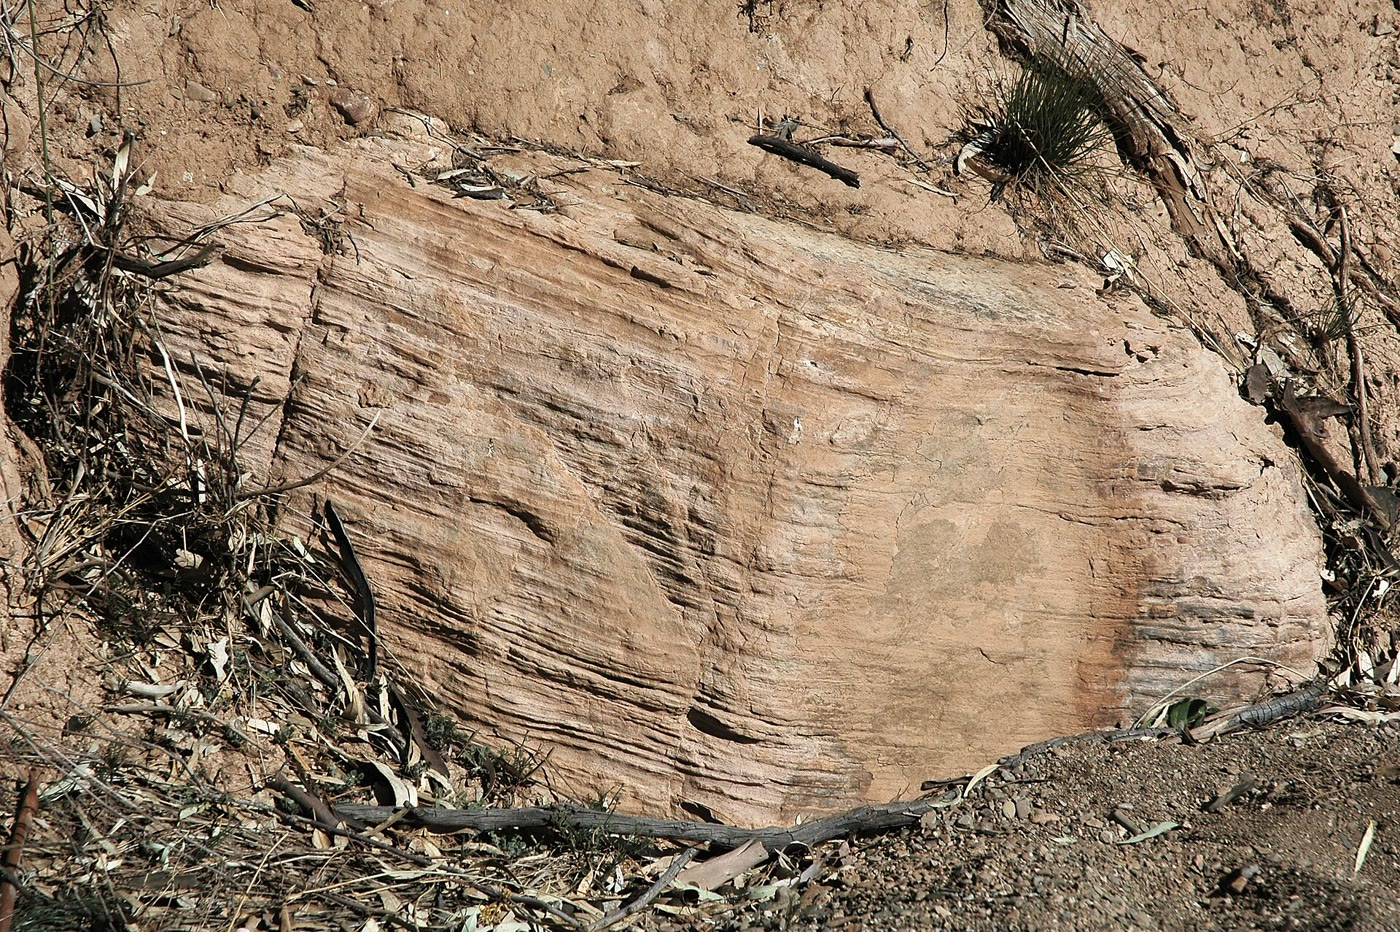
\includegraphics[width=0.66\linewidth]{images/book4/b2-18-cap-carbonate.jpg}
\par\smallskip{\small \omterm{def:b2:precambrian-earth:snowball}{Karbonat penudung}: batu dolomit berlaminasi Formasi Nuccaleena,
Flinders Ranges, Australia Selatan, yang bertumpu di atas endapan glasiasi Marinoan
(lapisan-lapisannya miring). Foto: James St.~John, CC~BY~2.0 (Wikimedia Commons).}
\end{omfigure}

Dua bola salju Kriogenian kini telah ditentukan umurnya dengan umur uranium--timbal pada zirkon dari abu
vulkanik dan dengan umur renium--osmium pada serpih yang kaya bahan organik. Sturtian dimulai antara 717.5 dan
\qty{716.3}{Ma} dan berakhir antara 659.3 dan \qty{658.5}{Ma}: \qty{58}{Ma} es, dengan
awal dan akhir yang serempak di seluruh dunia. Marinoan dimulai antara 649.9 dan
\qty{639.0}{Ma}, dengan penentuan umur yang longgar, dan berakhir antara 636.0 dan \qty{634.7}{Ma}: sedikitnya
\qty{3}{Ma}. Masing-masing berakhir dengan satu \omterm{def:b2:precambrian-earth:snowball}{karbonat penudung}, tidak pernah dengan beberapa. Formasi besi,
yang absen selama satu miliar tahun, kembali dalam endapan glasial Sturtian. Sedikitnya satu bola salju yang lebih awal,
di Siderian sekitar \qty{2.4}{Ga}, datang pada waktu GOE; di antara kedua
episode itu, selama sekitar \qty{1.5}{Ga}, hampir tidak ada lembaran es yang diketahui.
% ledger: hoffman17:ages, hoffman17:cryochrons, hoffman17:cap, hoffman17:models, hoffman17:earlier

\begin{history}[Dari hipotesis yang ganjil menjadi teori yang berumur pasti]
Pada 1964 W.~B. Harland menarik perhatian pada bukti glasiasi Prakambrium akhir. Pada
1968 dan 1969 M.~I. Budyko, dan W.~D. Sellers dengan model yang serupa, menemukan bahwa
\omterm{def:b2:precambrian-earth:ice-albedo}{umpan balik es--albedo} dapat membuat es menyebar sampai khatulistiwa begitu es itu maju cukup jauh; Bumi yang
membeku secara global ketika itu tampak sebagai keadaan tanpa jalan kembali, dan karena itu keadaan yang tidak pernah terjadi.
Pada 1981 J.~Walker, P.~Hays, dan J.~Kasting menguraikan termostat pelapukan silikat dan
mencatat bahwa di Bumi yang membeku karbon dioksida dari gunung api akan terakumulasi sampai es
mencair: keadaan itu dapat mengakhiri dirinya sendiri. Pada 1992 J.~L. Kirschvink mengajukan bahwa keadaan itu memang
pernah terjadi, dan menamainya ``Snowball Earth''; pada 1998 P.~F. Hoffman dan kawan-kawan menerbitkan
``A Neoproterozoic Snowball Earth'', dan epos-epos panglasial lalu disebut kriokron. Tidak ada
endapan glasial Kriogenian yang ditentukan umurnya secara radiometrik sebelum 2004; umur-umur di atas adalah
hasil kerja tahun-tahun sejak itu.
\end{history}
% ledger: hoffman17:history

Gunung api adalah jalan keluarnya. Di Bumi yang tertutup es, hujan dan sungai hampir berhenti, demikian pula pelapukan
silikat, dan karbon dioksida yang dilepaskan gunung api terakumulasi di udara
sampai efek rumah kacanya mencairkan es.

\begin{proposition}[Penumpukan karbon dioksida]\label{prop:b2:precambrian-earth:co2}
Jika karbon dioksida dilepaskan dengan laju $F$ (massa per tahun) ke dalam atmosfer bermassa
$M_{\text{a}}$ dan bermassa molar rata-rata $\bar M$, tanpa penyerap, waktu yang diperlukan untuk membawa rasio
pencampuran volumenya dari hampir nol sampai $x$ adalah
\[
  \tau = \frac{x}{1 - x}\,\frac{M_{\mathrm{CO_2}}}{\bar M}\,\frac{M_{\text{a}}}{F} .
\]
\end{proposition}

\begin{proof}
Atmosfer itu memuat $n = M_{\text{a}}/\bar M$ mol gas-gas lain. Menambahkan $n_c$ mol
karbon dioksida membuat rasio pencampurannya $x = n_c/(n + n_c)$, sehingga $n_c = n\,x/(1 - x)$, bermassa
$n_c M_{\mathrm{CO_2}}$; dengan laju $F$ hal ini memerlukan $\tau = n_c M_{\mathrm{CO_2}}/F$.
\end{proof}

\begin{example}[Berapa lama untuk lolos?]\label{ex:b2:precambrian-earth:escape}
Taksiran terpilih tertinggi untuk pelepasan vulkanik masa kini adalah \qty{0.26}{Gt} karbon
dioksida per tahun. Taksiran
rasio pencampuran yang diperlukan untuk mengakhiri bola salju Kriogenian berkisar dari 0.01 sampai 0.1. Dengan $M_{\text{a}} =
\qty{5.1e18}{kg}$, $\bar M = \qty{28.97}{g.mol^{-1}}$ dan $M_{\mathrm{CO_2}} =
\qty{44.01}{g.mol^{-1}}$, $x = 0.01$ memerlukan $\frac{0.01}{0.99}\times1.519\times\qty{5.1e18}{kg}
/ \qty{0.26e12}{kg.yr^{-1}} = \qty{0.30}{Ma}$, dan $x = 0.1$ memerlukan \qty{3.3}{Ma}.
\end{example}
% ledger: usgs:volcanic-co2, hoffman17:co2, earth:Matm, earth:Mmol, ciaaw:abridged-2024
% values: co2_t001_Myr 0.301, co2_t01_Myr 3.311 (precambrian.py)

Kolom karbon dioksida murni seberat \qty{1}{bar} di atas seluruh Bumi akan memerlukan
\qty{20}{Ma} dengan laju yang sama, angka yang diberikan Walker, Hays, dan Kasting. Beberapa juta tahun
itu lama, tetapi Sturtian berlangsung \qty{58}{Ma}. Entah ambangnya lebih tinggi, atau
pelepasan gasnya lebih rendah, atau Bumi yang membeku masih memiliki penyerap: pelapukan dasar laut muda,
yang tidak berhenti di bawah es, adalah salah satu kandidat. Dalam model neraca energi, lolosnya bola salju memerlukan
emisivitas efektif bola salju turun sampai suhunya mencapai \qty{263}{K}: di bawah
Matahari Kriogenian, \qty{94}{\percent} Matahari kini, dari 0.616 menjadi 0.472, pemerangkapan tambahan
sekitar \qty{39}{W.m^{-2}} (\cref{exo:b2:precambrian-earth:10}).
% ledger: hoffman17:co2, hoffman17:models, usgs:volcanic-co2
% values: one_bar_Myr 19.98, eps_melt_094 0.4716, forcing_melt_094 39.1 (precambrian.py)

Ketika es akhirnya terbuka di khatulistiwa, umpan balik itu berjalan mundur: laut yang gelap menyerap lebih banyak
sinar matahari, es mundur, dan model-model menunjukkan garis es yang melesat ke kutub dalam sekitar
\qty{2}{ka}. Bumi lalu mendapati dirinya dengan efek rumah kaca yang sangat besar di atas permukaan yang gelap, yaitu masa
sesudah yang panas. Pelapukan, yang sangat cepat dalam iklim itu, menuangkan kalsium, magnesium, dan bikarbonat ke dalam
laut, tempat \omterm{def:b2:precambrian-earth:snowball}{karbonat penudung} mengendap selagi air lelehan membanjiri paparan; diperlukan
sekitar sepuluh juta tahun untuk menarik turun kembali karbon dioksida itu. Lembaran es dan \omterm{def:b2:precambrian-earth:snowball}{karbonat
penudung}, formasi besi, dan umur-umur yang serempak adalah alasan sebagian besar ahli geologi kini menerima
bahwa bola salju Kriogenian memang terjadi, meskipun seberapa keras bola salju itu --- apakah sabuk air
terbuka bertahan di khatulistiwa, seperti yang diajukan model-model ``sabuk air'' --- masih diperdebatkan.
% ledger: hoffman17:hysteresis, hoffman17:cap, hoffman17:debate

\section*{Latihan}\label{sec:b2:precambrian-earth:exercises}

Data untuk latihan, kecuali dinyatakan lain: $\sigma = \qty{5.670e-8}{W.m^{-2}.K^{-4}}$;
$S_0 = \qty{1361}{W.m^{-2}}$; albedo kini 0.294 dan suhu permukaan rata-rata \qty{288}{K};
albedo bola salju 0.6; lereng dari \qty{263}{K} sampai \qty{283}{K}; emisivitas efektif kini
0.616; hukum Gough $L/L_0 = 1/(1 + 0.4\,t/t_\odot)$ untuk waktu $t$ sebelum kini, $t_\odot =
\qty{4.567}{Ga}$; likuidus \omterm{def:b2:precambrian-earth:greenstone}{komatiit} \qty{1616}{\celsius} pada \qty{32.2}{\percent} MgO,
kemiringan \qty{18.0}{\celsius} per persen; waktu paruh \ce{^{238}U} \qty{4.468}{Ga}, \ce{^{235}U}
\qty{0.704}{Ga}, \ce{^{232}Th} \qty{14.0}{Ga}, \ce{^{40}K} \qty{1.248}{Ga}.
% ledger: const:sigma, earth:TSI, earth:albedo, earth:Tsurf, hoffman17:models, gough81:luminosity, connelly12:cai, so16:liquidus, iaea:isotopes

\begin{exercise}[$\star$]\label{exo:b2:precambrian-earth:1}
(a) Berapa lama \omterm{def:b2:precambrian-earth:eons}{Hadean}, \omterm{def:b2:precambrian-earth:eons}{Arkean}, dan \omterm{def:b2:precambrian-earth:eons}{Proterozoikum} berlangsung? (b) Berapa fraksi umur
Bumi yang dibentuk oleh ketiganya bersama-sama? (c) Berapa umur Bumi ketika zirkon tertua yang diketahui
mengkristal, dan ketika batuan tertua terbentuk?
\end{exercise}

\begin{exercise}[$\star$]\label{exo:b2:precambrian-earth:2}
Kini \omterm{def:b2:elements-in-the-earth:bse}{Bumi silikat total} melepaskan, per kilogram, \qty{1.917}{pW} dari \ce{^{238}U},
\qty{0.082}{pW} dari \ce{^{235}U}, \qty{2.089}{pW} dari \ce{^{232}Th}, dan \qty{0.818}{pW} dari
\ce{^{40}K} ($\qty{1}{pW} = \qty{e-12}{W}$). (a) Tentukan masing-masing kontribusi \qty{3}{Ga} yang lalu, dan
totalnya. (b) Dengan faktor berapa produksi kalor telah turun sejak itu? (c) Isotop mana yang memimpin
kini, dan mana yang memimpin saat itu?
\end{exercise}

\begin{exercise}[$\star$]\label{exo:b2:precambrian-earth:3}
Gunakan termometer \omterm{def:b2:precambrian-earth:greenstone}{komatiit}. (a) Berapa likuidus \omterm{def:b2:precambrian-earth:greenstone}{komatiit} dengan
\qty{28}{\percent} MgO? (b) Kandungan MgO berapa yang sesuai dengan \qty{1500}{\celsius}? (c) Sebuah
aliran bertekstur spinifex memiliki MgO batuan utuh \qty{38}{\percent}. Mengapa likuidusnya tidak boleh
dibaca dari garis itu?
\end{exercise}

\begin{exercise}[$\star$]\label{exo:b2:precambrian-earth:4}
Susunlah berurutan dan berikan umur perkiraannya: \omterm{def:b2:precambrian-earth:goe}{Peristiwa Oksidasi Besar},
stromatolit yang pertama, akhir glasiasi Marinoan, \omterm{def:b2:precambrian-earth:greenstone}{komatiit} umum yang terakhir,
batuan tertua, kenaikan oksigen kedua, fosil Ediakaran pertama, akhir struktur kubah dan lunas
di Pilbara.
\end{exercise}

\begin{exercise}[$\star\star$]\label{exo:b2:precambrian-earth:5}
(a) Periksalah bahwa emisivitas efektif Bumi kini adalah 0.616. (b) Tentukan kesetimbangan bola salju
di bawah Matahari kini. (c) Tunjukkan bahwa kesetimbangan tengah, \qty{275.5}{K}, memenuhi
$R = E$ dalam selisih \qty{0.5}{W.m^{-2}}. (d) Tentukan kemiringan $R$ dan $E$ di situ, dan simpulkan
bahwa kesetimbangan itu tidak stabil.
\end{exercise}

\begin{exercise}[$\star\star$]\label{exo:b2:precambrian-earth:6}
(a) Dengan hukum Gough, tentukan sinar matahari \qty{2.4}{Ga} yang lalu dan \qty{0.65}{Ga} yang lalu sebagai fraksi
sinar matahari kini. (b) Dalam model itu, apakah iklim hangat mungkin pada setiap tanggal dengan emisivitas kini?
(c) Hoffman dan kawan-kawan menulis bahwa Matahari Siderian sekitar \qty{10}{\percent} lebih redup daripada
Matahari Kriogenian. Periksalah.
\end{exercise}

\begin{exercise}[$\star\star$]\label{exo:b2:precambrian-earth:7}
Sturtian berlangsung dari \qty{716.9}{Ma} sampai \qty{658.9}{Ma} (titik tengah selang yang ditentukan umurnya),
Marinoan dari \qty{644.5}{Ma} sampai \qty{635.4}{Ma}. (a) Tentukan lamanya masing-masing dan
masa antarglasial di antaranya. (b) Berapa fraksi periode Kriogenian, 720 sampai \qty{635}{Ma},
yang selama itu es menutupi Bumi, menurut angka-angka ini? (c) Mengapa lamanya Marinoan hanya merupakan angka
kasar?
\end{exercise}

\begin{exercise}[$\star\star$]\label{exo:b2:precambrian-earth:8}
(a) Berapa lama gunung api, dengan \qty{0.26}{Gt} per tahun tanpa penyerap, membawa udara ke
rasio pencampuran karbon dioksida 0.05? (b) Berapa kali \qty{278}{ppm} tahun 1750 nilai itu? (c) Jika separuh pelepasan itu diserap oleh pelapukan dasar
laut, berapa lama waktu yang diperlukan?
\end{exercise}
% ledger: usgs:volcanic-co2, earth:Matm, earth:Mmol, ciaaw:abridged-2024, ipcc:erf-2xco2

\begin{exercise}[$\star\star$]\label{exo:b2:precambrian-earth:9}
Sebuah diamiktit Neoproterozoikum mengandung batu-batu bergores, sebagian terletak dalam lumpur berlaminasi halus
yang melengkung ke bawah di bawahnya. (a) Apa yang ditunjukkan lengkungan itu? (b) Paleolintangnya adalah
\ang{10}. Mengapa hal ini penting bagi hipotesis bola salju? (c) Diamiktit itu langsung ditutupi oleh
batu dolomit berlaminasi yang berwarna merah muda dan setebal beberapa meter. Batuan apakah itu, dan apa yang direkamnya?
\end{exercise}

\begin{exercise}[$\star\star\star$]\label{exo:b2:precambrian-earth:10}
Di bawah Matahari Kriogenian, $S = 0.94\,S_0$. (a) Tunjukkan bahwa dalam model itu keadaan hangat masih
ada, nyaris, tetapi bola salju juga ada. (b) Tentukan suhu bola salju dengan
emisivitas kini. (c) Tentukan emisivitas yang membuat bola salju mencapai \qty{263}{K} dan
mencair. (d) Ubahlah perubahan emisivitas itu menjadi pemerangkapan tambahan radiasi gelombang panjang pada
\qty{263}{K}, dalam \unit{W.m^{-2}}.
\end{exercise}

\begin{exercise}[$\star\star\star$]\label{exo:b2:precambrian-earth:11}
(a) Dengan titik kritis \cref{prop:b2:precambrian-earth:tipping}, tunjukkan bahwa lebar
simpal histeresis, $S_{\text{m}}/S_{\text{f}}$, tidak bergantung pada emisivitas, dan
hitunglah. (b) Apa yang akan membuat simpal itu lebih sempit? (c) Mengapa bola salju hanya dapat mencair jauh dari
keadaan saat ia membeku?
\end{exercise}

\begin{exercise}[$\star\star\star$]\label{exo:b2:precambrian-earth:12}
Turunkan tetapan waktu model neraca energi di dekat kesetimbangan hangat, $\tau =
C/(E'(T^*) - R'(T^*))$, dan hitunglah nilainya untuk lapisan campuran samudra sedalam \qty{50}{m}, bermassa jenis
\qty{1025}{kg.m^{-3}} dan berkalor jenis \qty{3992}{J.kg^{-1}.K^{-1}}. Apa yang terjadi pada $\tau$ ketika
sinar matahari mendekati titik kritis kiri, dalam model ini dan dalam model yang albedonya berubah
secara mulus terhadap suhu?
\end{exercise}
% ledger: noaa:seawater-1025, teos10:cp0

\begin{problem}[{Soal akhir pekan --- Bumi muda yang lebih panas}]\label{pb:b2:precambrian-earth:1}
Soal ini mengikuti Bumi muda dari bagian dalamnya sampai udaranya. Gunakan data
latihan; \omterm{def:b2:elements-in-the-earth:bse}{Bumi silikat total} memuat \qty{0.0203}{ppm} uranium, \qty{0.0795}{ppm}
torium, dan \qty{240}{ppm} kalium menurut massa, dan isotop-isotopnya melepaskan \qty{95.13}{\micro W}
(\ce{^{238}U}), \qty{568.47}{\micro W} (\ce{^{235}U}), \qty{26.28}{\micro W} (\ce{^{232}Th}), dan
\qty{28.47}{\micro W} (\ce{^{40}K}) per kilogram isotop. Menurut massa, uranium terdiri atas
\qty{99.29}{\percent} \ce{^{238}U} dan \qty{0.711}{\percent} \ce{^{235}U}, dan kalium atas
\qty{0.0120}{\percent} \ce{^{40}K}. Bulatkan sampai tiga angka penting.

\noindent\textbf{Bagian I --- Kalor dari dalam.}
\begin{enumerate}
  \item Tentukan kalor yang dilepaskan kini oleh setiap isotop per kilogram \omterm{def:b2:elements-in-the-earth:bse}{Bumi silikat total}, dalam
        \unit{pW.kg^{-1}}.
  \item Tentukan totalnya.
  \item Tentukan tetapan peluruhan setiap isotop, dalam \unit{Ga^{-1}}.
  \item Tentukan masing-masing kontribusi \qty{2.7}{Ga} yang lalu, ketika \omterm{def:b2:precambrian-earth:greenstone}{komatiit} Pyke Hill dierupsikan.
  \item Tentukan totalnya saat itu, dan rasionya terhadap total kini.
  \item Isotop mana yang memberikan kalor terbanyak saat itu? Mengapa isotop itu memberikan begitu sedikit kini?
\end{enumerate}

\noindent\textbf{Bagian II --- Matahari Arkean.}
\begin{enumerate}[resume]
  \item Dengan hukum Gough, tentukan sinar matahari \qty{2.7}{Ga} yang lalu sebagai fraksi sinar matahari kini, dan dalam
        \unit{W.m^{-2}}.
  \item Tentukan kesetimbangan hangat pada sinar matahari itu dengan emisivitas kini. Apakah kesetimbangan itu merupakan keadaan hangat
        yang sah dalam model itu?
  \item Tentukan kesetimbangan bola salju pada sinar matahari itu.
  \item Emisivitas efektif berapa yang akan mempertahankan Bumi pada \qty{288}{K} dengan albedo hangat?
  \item Karbon dioksida saja dapat melakukannya dengan 0.004 sampai \qty{0.03}{bar} pada \qty{2.5}{Ga}.
        Dalam atmosfer sekitar \qty{1}{bar}, berapa kali \qty{278}{ppm} tahun 1750 nilai
        itu?
  \item Sebutkan proses yang menjaga karbon dioksida pada tingkat seperti itu selama ratusan juta
        tahun.
\end{enumerate}

\noindent\textbf{Bagian III --- Sebuah bola salju dan akhirnya.}
\begin{enumerate}[resume]
  \item Bola salju pertama, \qty{2.4}{Ga} yang lalu: tentukan sinar matahari saat itu sebagai fraksi sinar matahari kini.
        Apakah keadaan hangat model itu masih mungkin dengan emisivitas kini?
  \item Dengan \qty{0.26}{Gt} karbon dioksida per tahun, berapa lama waktu yang diperlukan untuk mencapai rasio
        pencampuran 0.1?
  \item Jika ambang di bawah Matahari Siderian yang lebih redup dua kali lebih tinggi, 0.2, berapa lama?
  \item Batuan mana yang merekam akhir sebuah bola salju, dan bagaimana?
  \item Mengapa formasi besi Sturtian memerlukan samudra tanpa oksigen di bawah es?
\end{enumerate}

\noindent\textbf{Bagian IV --- Termometer komatiit.}
\begin{enumerate}[resume]
  \item Periksalah kemiringan garis \omterm{def:b2:precambrian-earth:greenstone}{komatiit} dari kedua eksperimen.
  \item Cairan \omterm{def:b2:precambrian-earth:greenstone}{komatiit} Pyke Hill mengandung \qty{30}{\percent} MgO. Tentukan likuidusnya.
  \item Tentukan likuidus \omterm{def:b2:precambrian-earth:greenstone}{komatiit} Barberton, \qty{32.2}{\percent} MgO.
  \item Tentukan likuidus basal punggungan primer dengan \qty{12}{\percent} MgO.
  \item Dengan kemiringan Kilauea, \qty{20}{\celsius} per persen, sebagai gantinya, seberapa panas
        basal itu, mulai dari titik Barberton? Seberapa besar pengaruh pilihan kemiringan?
  \item Mengapa selisih suhu antara kedua lava lebih besar daripada selisih
        suhu potensial antara mantel \omterm{def:b2:precambrian-earth:eons}{Arkean} dan mantel kini?
  \item Sebagai ringkasan: seberapa jauh lebih panas lava \omterm{def:b2:precambrian-earth:greenstone}{komatiit} \omterm{def:b2:precambrian-earth:eons}{Arkean} terpanas daripada basal primer
        punggungan masa kini?
\end{enumerate}
\end{problem}
% ledger: ms95:pm-trace, dye:isotope-heat, iaea:isotopes, gough81:luminosity, cz20:archean-air, ipcc:erf-2xco2, usgs:volcanic-co2, hoffman17:co2, so16:liquidus, helz98:glass-thermometer, pierru22:komatiite
